\documentclass[conference,letterpaper]{IEEEtran}
\usepackage[T1]{fontenc}
\usepackage{amsmath,amssymb,graphicx,cite,url}
\urlstyle{rm}
\newcommand{\R}{\mathbb{R}}
\newcommand{\trans}{\mathsf{T}}
\title{Mechanical--Hydraulic Modeling of an\\Embankment Mower in Simscape}
\author{\IEEEauthorblockN{Kevin Kudakwashe Murera}
\IEEEauthorblockA{Robotics Research Lab, Department of Computer Science\\
RPTU Kaiserslautern-Landau\\Kaiserslautern, Germany}}
\pdfinfo{/Title (Mechanical-Hydraulic Modeling of an Embankment Mower in Simscape) /Author (Kevin Kudakwashe Murera)}
\begin{document}
\maketitle
\begin{abstract}
Hydraulic manipulators couple configuration-dependent mechanical loads with compressible-fluid dynamics and finite valve response. This project develops a Simscape model of the MULAG FME 500 embankment mower by combining CAD-derived geometry, a multibody mechanism, and valve-controlled hydraulic actuation. Cylinder geometry maps piston motion and axial force to joint motion and generalized torque. A joint-level feedback controller provides a repeatable trajectory-tracking task for studying plant sensitivity. Reported simulation results at four bulk moduli, from 0.5 to 2.0 GPa, show a decrease in the dominant joint's 50\% response delay from 847.4 to 649.7 ms and a decrease in end-effector RMS tracking error from 827.9 to 739.4 mm. The effects are not uniform: the fourth monitored joint's delay increases, while the mean tracking error is higher at the largest modulus than at the smallest. Numerical trajectory curves and tabulated results are preserved and redrawn as vector figures. The model supports virtual prototyping and control development; the available results establish simulation sensitivity rather than quantitative agreement with measured hardware. The report also identifies differences between the archived controller and the earlier written description so that future experiments can use a clearly specified implementation.
\end{abstract}
\begin{IEEEkeywords}
Hydraulic manipulator, multibody dynamics, Simscape, bulk modulus, trajectory tracking, virtual prototyping.
\end{IEEEkeywords}

\section{Introduction}
An embankment mower must position a cutting head through a long articulated mechanism while hydraulic actuators support gravitational, inertial, and external loads. An ideal joint-position or torque source is useful for kinematic analysis, but it does not represent pressure buildup, actuator compliance, flow limits, or valve dynamics. These effects matter when studying the time required to initiate motion and the error between a requested and realized cutting-head path.

Hydraulic control models commonly combine fluid continuity, pressure-dependent orifice flow, and actuator mechanics~\cite{merritt,jelali}. The modeling challenge is to connect these relations to the actual linkage geometry. A cylinder's moment arm changes with configuration, and motion of the linkage changes the fluid volume in each chamber. The resulting interaction is bidirectional: hydraulic force drives the mechanism, while mechanical motion changes chamber flow and pressure.

This project develops a coupled mechanical--hydraulic model of the MULAG FME 500 using MATLAB, Simulink, Simscape Multibody, and Simscape Fluids. The mechanical structure is derived from CAD and URDF assets; hydraulic actuators replace idealized actuation at the physical interface. A fixed joint-level controller is used to investigate the sensitivity of the simulated plant to bulk modulus. The contribution is the integrated modeling workflow and its documented sensitivity study, rather than a new controller stability theorem.

The report presents the geometry and governing relations, describes the archived implementation, and examines the numerical results. The supplied project contains the editable model, reference trajectories, analysis scripts, a presentation, and saved MATLAB figures. A matching earlier written report supplies additional methodological context. The numerical curves and summary tables are reused without claiming that new simulations or hardware tests were performed for this revision.

\begin{figure}[t]
\centering
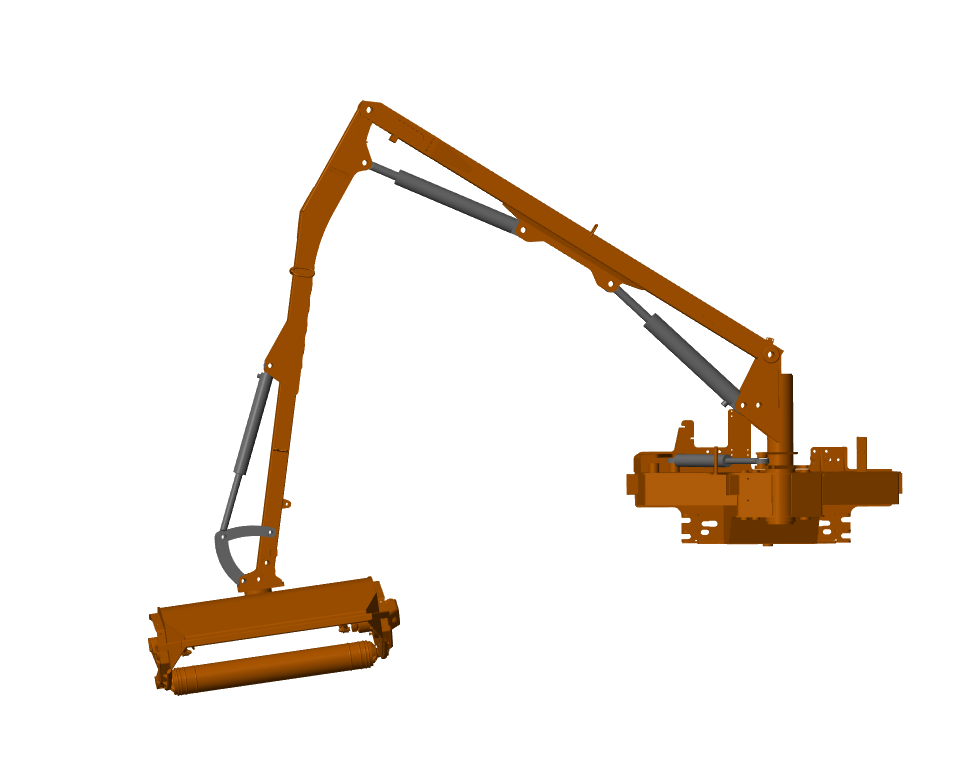
\includegraphics[width=.94\columnwidth]{../assets/Mulag_FME500.PNG}
\caption{CAD-derived visualization of the MULAG FME 500 mechanism supplied with the project. The independent arm coordinates are distinguished from the additional bodies and joints used to represent cylinder assemblies.}
\label{fig:robot}
\end{figure}

\section{Mechanical Model}
\subsection{Geometry and Model Import}
The arm is represented by five independent joint coordinates $q\in\R^5$. The project supplies several URDF descriptions: a six-link, five-revolute-joint representation for arm kinematics and a more detailed tree including actuator bodies. Extra joints in the detailed URDF are an import representation; they should not be interpreted as additional independently controlled arm degrees of freedom.

The CAD-to-URDF workflow provides link geometry, attachment frames, masses, and inertia tensors. URDF and rigid-body-tree models can be imported into Simscape Multibody using the supported model-import tools~\cite{smimport}. Inertial cross terms and the reference frame of each tensor must be preserved consistently. Geometry alone does not establish a measured mass distribution: density assignments, inertia reference frames, and imported units remain calibration inputs.

For a chosen external-wrench convention, the joint-space equations may be written
\begin{equation}
M(q)\ddot q+C(q,\dot q)\dot q+g(q)+\tau_f(\dot q)
=\tau_a+J_e(q)^\trans w_e,
\label{eq:mechanics}
\end{equation}
where $M$ is the inertia matrix, $C\dot q$ collects velocity-dependent terms, $g$ is gravity torque, and $w_e$ is the wrench applied by the environment to the end effector. The sign of the external term reverses if the opposite wrench convention is used. The model must use a consistent frame and sign convention throughout the physical interfaces.

\subsection{Cylinder Kinematics and Power Transfer}
Let $a(q)$ and $b(q)$ be the cylinder attachment positions in a common frame. The cylinder length, extension, and axial direction are
\begin{align}
\ell(q)&=\lVert b(q)-a(q)\rVert_2,\\
s(q)&=\ell(q)-\ell_0,\\
e_c(q)&=\frac{b(q)-a(q)}{\ell(q)}.
\end{align}
If $J_a$ and $J_b$ map joint velocities to attachment-point velocities, then
\begin{equation}
J_c(q)=e_c(q)^\trans[J_b(q)-J_a(q)],\qquad
\dot s=J_c(q)\dot q.
\end{equation}
Virtual work gives the generalized torque contribution
\begin{equation}
\tau_a=J_c(q)^\trans F_h.
\label{eq:force}
\end{equation}
This map preserves instantaneous mechanical power: $\tau_a^\trans\dot q=F_h\dot s$. For multiple cylinders, the scalar extension rows are stacked into a matrix. Geometry-dependent leverage is therefore included without assuming a constant force-to-torque ratio.

Cylinder attachments form closed mechanical loops in the assembled multibody model. The project describes spherical, prismatic, and cylindrical joint connections to provide axial extension and alignment freedom. Joint-frame inspection is essential because an incompatible connection can overconstrain a loop or change the sign of the actuator stroke. The earlier text also used an R--P--R description; the actual assembled joint topology should be taken from the selected model rather than assuming that the two descriptions are interchangeable.

\subsection{Hydraulic Stiffness in Joint Coordinates}
For a local closed-valve approximation with positive chamber volumes, the hydraulic contribution to axial stiffness is
\begin{equation}
k_h\simeq\beta_{\mathrm{eff}}
\left(\frac{A_A^2}{V_A}+\frac{A_B^2}{V_B}\right).
\end{equation}
The leading material-stiffness contribution in joint coordinates is
\begin{equation}
K_{q,\mathrm{mat}}\simeq J_c^\trans k_hJ_c.
\end{equation}
The complete derivative of~\eqref{eq:force} can also contain geometric-stiffness terms from the configuration dependence of $J_c$. Thus this expression is a local approximation, not a complete global stiffness matrix. Leakage, open valves, structural flexibility, and operating pressure alter the effective response.

The combination of slow arm motion and faster pressure dynamics can produce a stiff differential-algebraic system. The archived integrated model stores the implicit variable-step solver \textnormal{ode15s}; its stored relative tolerance is $10^{-3}$ and maximum step is 1.2~s. These are archived settings, not a verified accuracy recommendation. Step-size and tolerance convergence should be checked for each result~\cite{ode15s}.

\begin{figure*}[t]
\centering
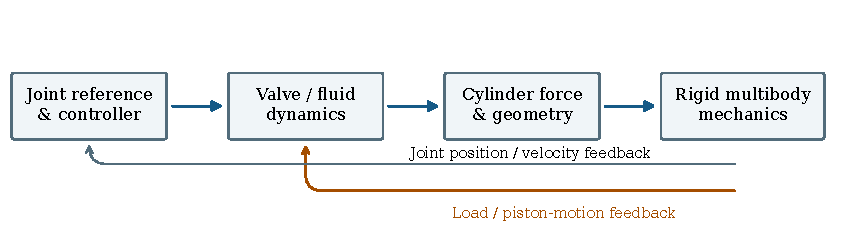
\includegraphics[width=\textwidth]{figures/coupled-architecture.pdf}
\caption{Functional organization of the coupled model. Cylinder motion changes chamber flow and pressure, while joint feedback closes the tracking loop. The diagram summarizes physical and signal relationships rather than reproducing every Simulink connection.}
\label{fig:architecture}
\end{figure*}

\section{Hydraulic Model}
\subsection{Supply and Fluid Compressibility}
The integrated model contains a fixed-displacement pump, pressure-relief elements, a gas-charged accumulator, directional valves, and double-acting actuators. The project presentation reports a nominal supply-flow scale of 40~L/min. A parameter helper specifies supply and tank pressures of 34 and 0.1~MPa, respectively; these helper values must not be assumed to override every block-level parameter.

For an ideal displacement pump,
\begin{equation}
Q_p=D_p\omega,
\end{equation}
when displacement $D_p$ is expressed per radian and $\omega$ in rad/s. If displacement is specified per revolution, the conversion must be included. An idealized accumulator gas law is $p_gV_g^\kappa=\mathrm{const}$ with absolute gas pressure $p_g$. Its effect depends on precharge, volume, and connection conditions.

Compressibility is described by an effective bulk modulus. A simple mixture approximation for liquid with local gas-volume fraction $\alpha$ is
\begin{equation}
\frac{1}{\beta_{\mathrm{eff}}}
\simeq\frac{1-\alpha}{\beta_\ell}
+\frac{\alpha}{\kappa p_{\mathrm{abs}}}.
\end{equation}
All terms have units of inverse pressure. This corrects the dimensionally incomplete volume-weighted expression in the earlier report. The sensitivity study varies a bulk-modulus parameter directly; it does not identify an entrained-air fraction from experiments.

\subsection{Valve Dynamics and Flow}
A first-order spool model describes finite valve response:
\begin{equation}
\tau_v\dot x_v=k_uu-x_v.
\end{equation}
Here $u$ is the electrical or normalized command and $k_u$ maps that command to spool displacement. This conversion is required if $u$ and $x_v$ have different units. The open flow path follows the signed orifice relation
\begin{equation}
Q=C_dA_o(x_v)\operatorname{sgn}(\Delta p)
\sqrt{\frac{2|\Delta p|}{\rho}}.
\end{equation}
The signed form allows pressure reversal. A 4/3 valve selects different supply and return paths for opposite spool directions; its metering area, leakage opening, and limits determine the flow behavior.

The integrated model uses Simscape Fluids isothermal-liquid blocks. Separate custom Simscape prototypes are also supplied. The custom valve uses a 0.07~s first-order command filter and a pressure-root flow law. These prototypes are retained separately because their legacy hydraulic-domain parameters are not automatically identical to the integrated isothermal-liquid implementation.

\subsection{Double-Acting Cylinder}
For extension coordinate $s$, define
\begin{equation}
V_A=V_{A0}+A_As,\qquad
V_B=V_{B0}+A_B(L-s).
\end{equation}
With $Q_A$ positive into chamber A, $Q_B$ positive out of chamber B, and internal leakage $Q_\ell=C_\ell(p_A-p_B)$, continuity gives
\begin{align}
\dot p_A&=\frac{\beta_{\mathrm{eff}}}{V_A}
(Q_A-A_A\dot s-Q_\ell),\\
\dot p_B&=\frac{\beta_{\mathrm{eff}}}{V_B}
(-Q_B+A_B\dot s+Q_\ell).
\end{align}
The pressure-force relation is
\begin{equation}
F_h=A_Ap_A-A_Bp_B-F_f(\dot s).
\end{equation}
Area asymmetry, dead volume, and piston motion affect the chamber pressures; these are also explicit features of the standard double-acting actuator formulation~\cite{actuator}.

One regularized viscous/Coulomb friction model is
\begin{equation}
F_f(v)=b_vv+F_c\tanh(v/v_\epsilon).
\end{equation}
The archived custom cylinder implements this form with an optional efficiency multiplier. It does not implement the full Stribeck curve claimed in the earlier text. Likewise, its chamber equations omit an explicit internal-leakage term. The general equations above describe the modeling framework; individual block settings determine which effects are active in a selected implementation.

\section{Trajectory and Feedback Control}
\subsection{Reference Generation}
The reference pipeline uses a rigid-body representation and inverse kinematics to generate joint positions, velocities, accelerations, and an end-effector path. The project includes an arc-and-chord trajectory generator as well as a separate mowing-sweep example. These are different reference-generation examples and should not be treated as one experiment.

The integrated model's Signal Editor blocks read the supplied joint-position, joint-velocity, joint-acceleration, and end-effector MAT datasets. The organized project retains these files without altering their numerical content. The stored input sample times are 0.005~s for position, velocity, and end-effector references and 0.01~s for acceleration. Dataset timing and controller execution must be checked together before a new run.

\subsection{Archived Controller Structure}
The original report describes integral backstepping on every axis. The embedded controller in the archived integrated model is more specific: joints 1, 3, 4, and 5 use a backstepping-inspired error law, while joint 2 uses position PI, velocity feedback, gravity bias, and a soft limit term. Pressure and supply-pressure ports are present but unused by that function.

For the four backstepping branches,
\begin{align}
z_{1,i}&=q_{r,i}-q_i,\\
\alpha_i&=\dot q_{r,i}+c_{1,i}z_{1,i},\\
z_{2,i}&=\alpha_i-\dot q_i,\\
I_i^+&=\operatorname{clip}(I_i+T_sz_{2,i},-I_{\max,i},I_{\max,i}),\\
u_{b,i}&=\frac{z_{1,i}+c_{2,i}z_{2,i}+K_{I,i}I_i}{b_i}.
\end{align}
Integration is gated when the previous command approaches saturation. A friction-bias term is added above a small error threshold; actuator sign and command bias are then applied before clipping. This practical error-feedback law is not accompanied by a Lyapunov proof for the full coupled plant.

Joint 2 instead uses
\begin{equation}
u_{\mathrm{PI},2}=K_pe_2+K_iI_2+K_v(\dot q_{r,2}-\dot q_2),
\end{equation}
with $K_p=1200$, $K_i=3$, and $K_v=4$. A configuration-dependent bias $0.40\cos q_2+0.25\cos(q_2+q_3)$ and a soft position-limit contribution are added before actuator mapping and saturation. These are command-space gains and biases; they are not identified physical torque parameters.

\begin{table}[t]
\caption{Embedded Controller Settings for Backstepping Branches}
\label{tab:gains}
\centering
\begin{tabular}{rrrrrr}
\hline
Joint & $c_1$ & $c_2$ & $K_I$ & $b$ & $|u|_{\max}$\\\hline
1 & 800 & 1 & 1.5 & 8 & 0.95\\
3 & 6 & 1.5 & 2 & 12 & 0.80\\
4 & 800 & 1 & 2 & 10 & 0.80\\
5 & 6 & 1.5 & 1 & 15 & 0.90\\\hline
\end{tabular}
\end{table}

The embedded integration interval is $T_s=0.005$~s, rather than the 0.01~s stated in the earlier report. The model's separate error-accumulation helper contains 0.01~s. The offline metric function uses the actual recorded time vector and trapezoidal integration, which avoids silently assigning the controller's interval to every log.

\begin{figure*}[t]
\centering
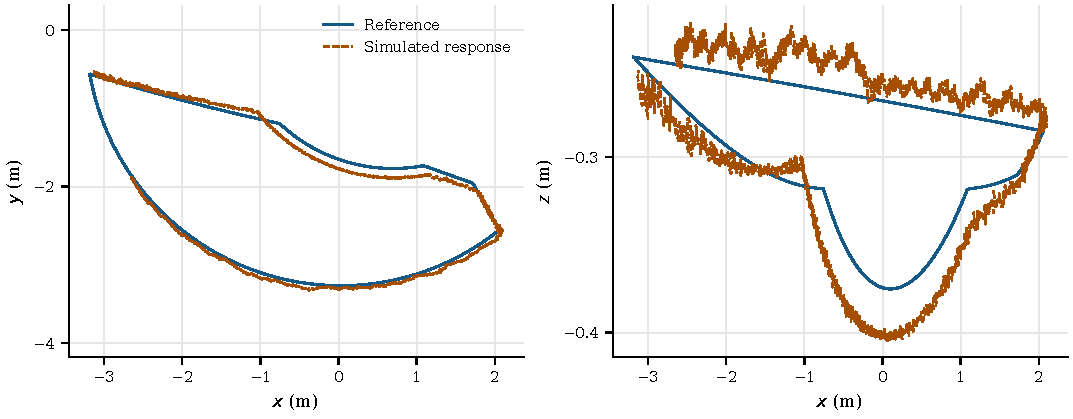
\includegraphics[width=\textwidth]{figures/task-space-path.pdf}
\caption{Archived task-space reference and simulated response, redrawn directly from numerical curves in \textnormal{plot.fig}. Left: horizontal projection; right: vertical projection. The two curves contain 3,991 and 3,550 samples, respectively, and no shared time vector is stored with these extracted coordinates. This figure is a historical simulation visualization, not a new run or a recomputed tracking-error measurement.}
\label{fig:path}
\end{figure*}

\section{Evaluation Method}
\subsection{Threshold-Based Response Timing}
The MATLAB analysis function monitors four channels using valve command, cylinder extension, chamber pressures, and joint position. Command onset $t_0$ is the first threshold crossing of $|u(t)-u(0)|$, with threshold equal to the larger of 5\% of the command span and an absolute value of 0.002 in the command's units. This is distinct from the 50\% criterion used for the response signals.

For a response $r$, the analysis finds the first post-onset crossing of
\begin{equation}
|r(t)-r(0)|=0.5\max_{t\geq t_0}|r(t)-r(0)|.
\end{equation}
Cylinder extension, differential pressure, and joint position define times $t_x$, $t_p$, and $t_q$. The principal intervals are
\begin{equation}
\tau_{v\to x}=t_x-t_0,\quad
\tau_{v\to p}=t_p-t_0,\quad
\tau_{v\to q}=t_q-t_0.
\end{equation}
Crossings are linearly interpolated between recorded samples. This improves the numerical crossing estimate without creating independent sub-sample measurement resolution. If a response is already above threshold at the first retained post-onset sample, the implementation uses that sample's time.

The quantity $\tau_{v\to q}$ is a threshold-based rise-response interval. It combines command dynamics, pressure response, reference shape, controller action, and mechanical motion; it is not a separately identified pure transport delay. Nonmonotone trajectories and small-amplitude axes require care in interpreting their first crossing.

For four available joint intervals, the reported aggregate is
\begin{equation}
\tau_{\mathrm{RMS}}=\sqrt{\frac14\sum_{j=1}^{4}\tau_{v\to q,j}^{\,2}}.
\end{equation}
An undefined or unexcited response should be marked missing and reported with its valid count. It must not be silently replaced by a zero-delay measurement.

\subsection{Task-Space Error}
For synchronized reference and response positions,
\begin{equation}
e(t)=\lVert p_r(t)-p(t)\rVert_2.
\end{equation}
On a declared active window of duration $T$,
\begin{align}
E_{\mathrm{RMS}}&=\sqrt{\frac1T\int_{t_s}^{t_e}e(t)^2\,dt},\\
E_{\mathrm{mean}}&=\frac1T\int_{t_s}^{t_e}e(t)\,dt.
\end{align}
The offline function begins at the earliest valid command onset and uses time-weighted trapezoidal integration. A variable-step solver makes time weighting particularly relevant. The archived spatial curves in Fig.~\ref{fig:path} have different sample counts and lack a shared time base; indexwise subtraction of these extracted curves would therefore not reproduce these metrics.

\begin{figure*}[t]
\centering
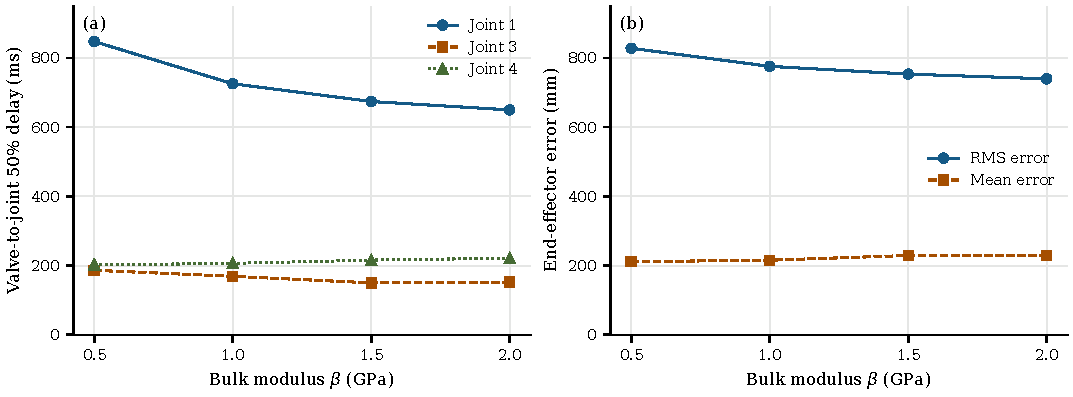
\includegraphics[width=\textwidth]{figures/bulk-modulus-sensitivity.pdf}
\caption{Reported bulk-modulus sensitivity redrawn from the numerical values in the original analysis script and report. (a) Joint-specific 50\% response intervals. (b) RMS and mean end-effector errors. Markers denote the four reported cases; connecting lines guide the eye and are not extra simulated cases.}
\label{fig:sensitivity}
\end{figure*}

\section{Results and Discussion}
\subsection{Available Numerical Evidence}
The four reported cases use $\beta\in\{0.5,1.0,1.5,2.0\}$~GPa. Table~\ref{tab:results} and Fig.~\ref{fig:sensitivity} reproduce the supplied numerical summaries. The chosen joint-delay values agree between the source presentation, Table~I of the earlier report, and \textnormal{delaysvserror.m}. Table~II of the earlier report gives a different set of joint-3 intervals; those conflicting values are not combined with the consistent series. The disagreement is recorded in the repository's data-provenance notes.

\begin{table*}[t]
\caption{Reported Simulation Summary Across Bulk-Modulus Cases}
\label{tab:results}
\centering
\begin{tabular}{rrrrrrr}
\hline
$\beta$ (GPa) & Joint 1 (ms) & Joint 3 (ms) & Joint 4 (ms) & Reported $\tau_{\mathrm{RMS}}$ (ms) & $E_{\mathrm{RMS}}$ (mm) & $E_{\mathrm{mean}}$ (mm)\\\hline
0.5 & 847.4 & 186.3 & 202.1 & 445.4 & 827.9 & 211.3\\
1.0 & 725.3 & 168.8 & 206.4 & 386.4 & 775.6 & 215.4\\
1.5 & 674.0 & 149.9 & 215.8 & 361.7 & 753.2 & 229.1\\
2.0 & 649.7 & 152.4 & 221.6 & 351.6 & 739.4 & 228.8\\\hline
\end{tabular}
\end{table*}

\subsection{Joint-Specific Trends}
Joint 1 has the largest reported response interval. Raising the bulk modulus from 0.5 to 2.0~GPa reduces that interval by 197.7~ms, or approximately 23.3\%. The reported aggregate decreases by 93.8~ms, approximately 21.1\%. Most of the reduction occurs below 1.5~GPa in these four cases.

The other joints do not follow an identical trend. Joint 3 decreases from 186.3 to 149.9~ms at 1.5~GPa, then rises to 152.4~ms. Joint 4 increases from 202.1 to 221.6~ms, about 9.6\%. This nonuniform behavior is consistent with the fact that a threshold interval depends on the coupled plant, feedback law, and trajectory. The results do not support claiming that every axis becomes faster as fluid stiffness increases.

The earlier report states that joint 2's interval remains below 0.3~ms. Its four individual values are not included in the summary script. The aggregate can be approximated to the displayed precision by setting this small contribution to zero; however, that arithmetic is not evidence of a truly instantaneous joint response. It also cannot establish a valve bandwidth from signals sampled on a coarser grid.

\subsection{Tracking-Error Trends}
The reported RMS end-effector error falls from 827.9 to 739.4~mm, a reduction of 88.5~mm or approximately 10.7\%. The mean error does not improve in parallel: it changes from 211.3 to 228.8~mm, approximately 8.3\% higher at the largest modulus. The earlier statement that the mean error follows the same improving pattern is therefore incorrect.

RMS and mean error emphasize different parts of a trajectory. A lower RMS with a higher mean is mathematically possible, for example when large transient errors decrease while a smaller persistent error increases. The available summary values alone do not establish which time segments cause the difference. Their relatively large RMS-to-mean ratios motivate inspecting synchronized error histories, initialization, and the active integration window in future runs.

The largest reported RMS error is about 0.83~m and the smallest about 0.74~m. These values should be presented with their physical scale; they do not justify an unqualified claim of high-precision mowing. The spatial view in Fig.~\ref{fig:path} helps illustrate the trajectory, but it cannot replace quantitative error analysis.

\subsection{Scope of Validation}
The sweep establishes sensitivity of the simulated closed-loop system to a selected parameter. It does not independently verify that chamber pressures, friction, cylinder forces, and end-effector motion match a physical mower. The archive supplies no synchronized hardware measurements or parameter-identification uncertainty bounds for such a comparison.

Similarly, the smooth normalized step responses in the original \textnormal{delay\_plots.m} script are generated from an assumed second-order model, fitted to reported crossing times. They are explanatory reconstructions, not raw hydraulic-simulation traces. They remain in the archive but are excluded from the revised report's result figures. The separate custom components and parameter helpers describe additional configurations; their constants should not be mixed with the integrated model's blocks as if all came from one run.

\section{Reproducibility and Further Work}
The organized repository separates the editable integrated model, earlier model variants, physical source components, canonical geometry, reference datasets, numerical plot exports, and documentation. Repeated mesh copies, simulation caches, autosaves, generated native binaries, and Blender backups are excluded from active source. The full original GitLab archive is retained as a release asset, with source hashes and a migration map.

The imported model was saved in MATLAB R2023b. Absolute Windows geometry references and Signal Editor file references are replaced by project-relative paths. The model's equations, controller code, and solver settings are preserved. The setup function adds the relevant folders to the MATLAB path and directs regenerated cache/code-generation files to a separate build directory. The revised documentation opens the editable \textnormal{.slx} model rather than a \textnormal{.slxc} simulation cache.

Artifact checks verify retained-file hashes, model-archive integrity, geometry and input-file references, URDF mesh resolution, numeric-curve exports, report tables, and documentation links. They do not replace loading and running the project in a licensed MATLAB installation. No end-to-end MATLAB simulation or hardware test was conducted for this revision.

Further work should first establish one versioned model configuration and timing contract. A reproducible sweep should save the controller gains, active block parameters, solver settings, reference trajectory, all event signals, and synchronized end-effector errors for each case. Tolerance studies should demonstrate convergence of the reported metrics. Physical validation should then compare measured and simulated pressure, stroke, force, and motion under matched inputs before the model is described as a calibrated digital twin.

\section{Conclusion}
The project couples a CAD-derived multibody arm with hydraulic supply, valve, and cylinder dynamics for virtual prototyping of an embankment mower. Geometry-dependent force transmission and fluid continuity connect the two physical domains. The reported parameter sweep shows that larger bulk modulus reduces the dominant joint's response interval and end-effector RMS error for the supplied task, while other joint intervals and mean error behave differently. These results motivate evaluating several metrics together and retaining the complete experimental configuration. The organized model and numerical assets provide a documented basis for further simulation, identification, and control development; agreement with physical hardware remains a separate validation task.

\section*{Acknowledgment}
This project was carried out at the Robotics Research Lab, RPTU Kaiserslautern-Landau.

\bibliographystyle{IEEEtran}
\bibliography{references}
\end{document}
